\documentclass[../main.tex]{subfiles}

\begin{document}

    \chapter{Inferència causal} \label{ch:intro}
    
    L’objectiu de la inferència causal és explorar una possible causa d’un fenomen. Això es fa avaluant si una intervenció (com un tractament mèdic, una campanya publicitària o una política pública) és la responsable d’un determinat resultat, és a dir, estimant l’efecte de la intervenció. Paral·lelament, per entendre de què estem parlant, és essencial comprendre què significa realment el concepte de causalitat.
    \linebreak
    Segons la RAE, una causa és "allò que es considera com a fonament o origen d’alguna cosa". Tanmateix, en la ciència, la determinació de relacions causals no és tan senzilla. Abans d’entrar en detall en el treball, primer hem d'entendre com l’estadística aborda la causalitat i quins són els desafiaments que implica.

    
    \section{Correlació no implica causalitat}\label{sec:cor_no_causalitat}
    Un dels principis fonamentals de l’estadística és: “correlació no implica causalitat”. Això significa que el fet que dues variables es moguin conjuntament no vol dir necessàriament que una sigui la causa de l’altra. \par
    Per exemple, podem observar que el consum de gelats i el nombre d’ofegaments augmenten durant l’estiu. Tot i que hi ha una correlació clara entre aquestes dues variables, això no significa que menjar gelat causi ofegaments. En realitat, existeix una tercera variable latent -la temperatura o època de l'any- que afecta ambdues variables i explica la relació observada.\par
    Aquest tipus d’associacions espúries evidencien la necessitat d’eines estadístiques més avançades per inferir relacions causals de manera rigorosa. La inferència causal pretén identificar si una relació observada és realment causal o només una coincidència resultat de factors ocults. Així, en comptes de basar-nos només en correlacions, aquests models ens ajuden a establir relacions de causa-efecte.\par
    Més enllà de la correlació, les regressions poden ser una eina molt útil per analitzar relacions entre variables, donen informació de com varia un resultat en funció d’altres variables. Doncs, les regressions són una forma senzilla i bàsica d’apropar-nos a la causalitat; no obstant això, també poden ser perilloses si el model no està correctament especificat. Una mala especificació pot portar-nos a identificar erròniament una causa o, al contrari, a descartar-ne una de real. A més, fins i tot amb un model ben especificat, la qualitat de les conclusions depèn de les dades disponibles. Si el conjunt de dades prové d’un mal disseny experimental o conté limitacions inherents, els resultats poden ser enganyosos i portar a conclusions incorrectes. Doncs, la regressió és un bon mètode per predir una variable, però abans s’ha de tenir clar els mecanismes de causalitat que lliguen les variables.

    \section{Assumpcions bàsiques}\label{sec:assumpcions}
    Per poder fer inferència causal, és a dir, calcular l’efecte d’un tractament, s’ha de complir tres condicions bàsiques, seguint a \citep{abecassis2024}:
    \begin{enumerate}
        \item \textbf{STUVA (Stable Unit Treatment Value Assumption) o Consistència:} L’outcome d’una unitat no depèn del de cap altra unitat, no hi ha influència entre unitats , i només existeix una versió del tractament al que ens referim.
        \begin{equation}
            Y(a)=Y\qquad si\;\,\,A=a
        \end{equation}
        
        \item \textbf{Ignorabilitat}: L’assignació d’un tractament es independent del potencial del outcome, si fa falta després de condicionar per algunes variables. De manera que podríem considerar com si fos una assignació aleatòria.
        \begin{equation}
            Y(0),Y(1)\perp A
        \end{equation}
        En el cas que estiguem condicionant per algunes variables, és a dir, treballant amb una visió més individualitzada i centrant-nos en els efectes heterogenis del tractament, aquesta assumpció es pot expressar com:
        \begin{equation}
            Y(0),Y(1)\perp A\,\mid\,X=x_i
        \end{equation}
        Aquesta formulació implica que, un cop controlem per les covariables X, l’assignació al tractament és independent dels outcomes potencials. És a dir, estem suposant que no hi ha biaix de confusió: qualsevol variable que pogués afectar tant l’assignació al tractament com el resultat ja està recollida a X. Això ens permet estimar de manera vàlida l’efecte causal fins i tot en contextos amb heterogeneïtat

        \item \textbf{Overlap o positivitat}: Totes les unitats tenen una probabilitat estrictament positiva a estar en qualsevol dels grups de tractament.
        \begin{equation}
            0<P(A=a)<1 \qquad \qquad \text{sent \textbf{a} qualsevol dels tractaments possibles}
        \end{equation}
        Aquesta assumpció també té una versió que s’ha de respectar per treballar amb efectes heterogenis:
        \begin{equation}
            0<P(A=a\;\mid\; X=x_i)<1 \qquad \qquad \text{sent \textbf{a} qualsevol dels tractaments possibles}
        \end{equation}
        És a dir, tots els diferent nivells pels que decidim condicionar han de tenir una probabilitat de rebre el tractament diferent de 0 i de 1.
    \end{enumerate}
    
    Les tres assumpcions bàsiques són essencials per poder identificar l’efecte mitjà del tractament (vegeu la secció \ref{sec:ate}), i les seves versions condicionades són igualment fonamentals quan es treballa amb l’efecte causal condicional mitjà (CATE). Com ja hem comentat, a l’hora d’estudiar efectes heterogènis del tractament, cal tenir molt present la versió condicionada d’aquestes assumpcions i escollir acuradament les variables sobre les quals condicionarem. Aquesta elecció determina com podem estratificar la població, el que tindrà molt d'impacte en la validesa de les estimacions, ja que és una manera de controlar els factors de confusió rellevants. \cite{hernan2020}

    \section{Efecte mitjà del tractament}\label{sec:ate}
    L’ATE, o Efecte Mitjà del Tractament, mesura l’impacte mitjà d’una intervenció o tractament sobre una població. Aquest efecte es calcula com la diferència entre el valor esperat de l'outcome (resultat) quan es rep el tractament i quan no es rep. Si suposem que el tractament és binari ($T\in\{0,1\}$), l’ATE es defineix com: \citep{hernan2020}
    \begin{equation}
        ATE=\mathbb{E}[\mathbb{E}[Y\,\mid\,T=1]-\mathbb{E}[Y\,\mid\,T=0]]
    \end{equation}
    El principal desafiament de la inferència causal és que, en la majoria dels casos, no podem observar simultàniament l'outcome d’un individu amb i sense tractament \citep{Holland1986}. Sovint és materialment impossible que una mateixa persona pertanyi simultàniament a dos grups (tractament i control). A més, en dades observacionals, normalment no tenim assignació aleatòria del tractament, cosa que pot portar a desbalanceig entre els diferents grups.
    Per abordar aquest problema, introduïm el concepte de resultats potencials ($Y_1,Y_0$), que representen els valors que prendria l'outcome en cadascun dels dos escenaris possibles:
    \begin{itemize}
        \item  $Y_1$: el resultat si l’individu rep el tractament (T=1).
        \item $Y_0$ el resultat si l’individu no rep el tractament (T=0).
    \end{itemize}
    L'ATE es pot redefinir en termes d’aquests resultats potencials com:
    \begin{equation}
        ATE=\mathbb{E}[Y_1]-\mathbb{E}[Y_0]
    \end{equation}
    Aquesta formulació ens permet entendre que el gran repte de la inferència causal és estimar aquests valors contrafactuals, és a dir, els resultats que no s'han observat perquè un individu només pot rebre un dels dos tractaments possibles.\par
    Més endavant veurem com el Conditional Average Treatment Effect està a la base de l’Heteregeniuos Tractment Efect, és a dir, és la versió de l'ATE quan ho mirem d’una forma més individualitzada, condicionant per altres variables de $X$.


    \section{Propensity Score}\label{sec:ps}
    Molt relacionat amb els resultats potencials, trobem el concepte de propensity score, que representa la probabilitat que una unitat rebi el tractament donades les seves característiques. Aquesta idea neix de la intuïció que no cal condicionar directament per totes les covariables X per garantir la independència entre el tractament T i els resultats potencials ($Y_0, Y_1$). En lloc d’això, n'hi ha prou amb balancejar el tractament en funció del propensity score, de manera que l'esperança condicional $E[Y\,\mid\,T]$ sigui comparable entre grups. \citep{facure2022} \par
    Formalment, el propensity score s’expressa com:
    \begin{equation}
        e(x_i)=P(T\,\mid\,X)
    \end{equation}
    És a dir, la probabilitat que la unitat amb característiques $X_i$ rebi el tractament.
    Com que es tracta d’una probabilitat que cal estimar, hi ha diverses maneres de fer-ho, des de regressions logístiques tradicionals fins a mètodes d’aprenentatge automàtic com els random trees, random forests o xarxes neuronals. 
    Aprofitant que el propensity score $e(x)$ encapsula tota la informació de X rellevant per a l’assignació al tractament, podem afirmar que $\mathbb{E}[T\,\mid\,e(X),X]=\mathbb{E}[T\,\mid\,e(X)]$ \par
    Aquesta propietat ens indica que el propensity score és un resum suficient de les covariables $X$ pel que fa a la probabilitat de rebre el tractament $T$. Un cop sabem $e(x)$, la informació de $X$ ja no aporta res addicional sobre T.
    Aquesta idea és fonamental en inferència causal, ja que sota la suposició d’ignorabilitat condicional (és a dir, $(Y_0,Y_1)\perp T\,\mid\,X$), es pot demostrar que també es compleix: $(Y_0,Y_1)\perp T\,\mid\,e(x)$ \par
    Això vol dir que, condicionant pel propensity score, podem tractar l'assignació al tractament com si fos aleatòria, i per tant podem estimar l’efecte causal sense haver de condicionar per totes les covariables $X$. En conclusió, ens permet reduir la dimensionalitat del problema, passant d’una gran quantitat de covariables $X$ a una sola funció escalar $e(x)$, mantenint la validesa.
    
    \subsection{Utilitats}\label{subsec_ps:utilitat}
    Òbviament el càlcul del PS van més enllà de simplement tenir una informació de la probabilitat de rebre el tractament per cada individu. Això ens serveix intentar fer una espècie de balanceig per aïllar més l’efecte de la intervenció i, per tant, guanyar validesa. Podem fer: \citep{austin2011}
    \begin{itemize}
        \item \textbf{Matching:} Consisteix a emparellar unitats tractades i no tractades segons la seva proximitat en el PS. Aquest emparellament es pot fer amb diferents criteris, com per exemple 1:1 matching, matching amb reemplaçament, o amb una certa tolerància (caliper). Un cop formats els grups amb la metodologia escollida, es comparen els outcomes entre les unitats tractades i les no tractades emparellades per estimar l'efecte del tractament.
        \item \textbf{Estratificació:} És una estratègia similar al matching, però en lloc d’emparellar unitats individualment, es divideixen totes les unitats en estrats (o grups) segons el valor del propensity score —sovint utilitzant quantils com quintils o decils. Dins de cada estrat, es comparen els outcomes entre unitats tractades i no tractades. Finalment, les diferències obtingudes en cada estrat es combinen, ponderant-les segons la mida de cada estrat, per estimar l’efecte global del tractament.
        \item \textbf{Ajustament per covariables:} D’entre els quatre mètodes, aquest és l’únic que es basa en un model de regressió. El model es construeix utilitzant el propensity score com a covariable, habitualment juntament amb la variable de tractament, per predir l’outcome. Així, el coeficient estimat de la variable de tractament ens dona una estimació de l’efecte causal, ja que el propensity score hauria capturat les possibles fonts de confusió presents en les covariables originals.
        \item \textbf{IPTW:} Sigles amb anglès de Inverse Probability of Treatment Weighting com el seu nom indica, aquest mètode utilitza el PS per assignar pesos a les observacions segons la probabilitat de rebre el tractament. Una forma habitual de calcular aquests pesos és:\\
        $w_i=\frac{T_i}{e(x_i)}+\frac{(1-T_i)}{(1-e_i)}$\\
        on $T_i$ és la variable de tractament (0 o 1) i $e(x_i)$ és el propensity score de la unitat i. Un cop assignats els pesos, es pot calcular una tipus de mitjana ponderada dels outcomes per estimar l’efecte del tractament. Aquest mètode crea una “pseudopoblació” en què l’assignació al tractament és independent de les covariables. Més endavant, veurem com aquest esquema s'utilitza dins d’alguns meta-learners, com el X-learner.
    \end{itemize}

    
    \section{Grafs causals}\label{sec:dag}
    Per comprendre com funciona la causalitat en un context específic, és molt útil utilitzar un Diagrama Acíclic Dirigit (DAG, per les seves sigles en anglès). Aquest tipus de representació visual ens ofereix una manera clara de veure les relacions entre les variables, ajudant-nos a identificar els elements clau abans de començar a modelitzar. \par
    A més, el DAG permet visualitzar de manera senzilla com es transmet la causalitat i la dependència entre les diferents variables, facilitant la identificació del rol que cada una d'elles juga en el sistema. Aquesta representació també ens ajuda a entendre quines variables poden influir en altres i com aquestes interaccions afecten el resultat final. Els tres casos més fonamentals per entendre el paper de les variables que no són Intrevenció/Tractament o Resposta són els següents: (a la següent taula \ref{taula:path} amb il·lustracions de Neal (2020) estan representades en un DAG)
    \begin{itemize}
        \item \textbf{Collider:} es produeix quan dues variables independents causen un resultat comú, reb causes des de dos variables. Podem obrir un camí causal entre les dues variables independents.
        \item \textbf{Mediadora:} és una variable que explica el mecanisme pel qual una variable independent causa un resultat. És a dir, la variable mediadora transmet l'efecte de la variable causal a la variable resultat. Si condicionem sobre la mediadora, podem bloquejar el camí causal, fent que es perdi la connexió entre la causa i el resultat.
        \item \textbf{Confusora:} és una variable que afecta tant a la variable causal com al resultat, creant una relació espúria entre elles. Una confusora pot introduir un biaix en l'estimació de l'efecte causal si no es controla/condiciona, ja que pot fer que sembli que hi ha una relació causal entre la variable causal i el resultat quan, en realitat, la relació és deguda a la confusora.
    \end{itemize}

    \begin{table}[h] 
    \centering
    \renewcommand{\arraystretch}{1.5}
        \begin{tabular}{>{\raggedright}m{2.5cm} 
                        >{\centering\arraybackslash}m{3.5cm} 
                        >{\centering\arraybackslash}m{3.5cm} 
                        >{\centering\arraybackslash}m{3.5cm}}
        
        \toprule
         & \textbf{Collider} & \textbf{Mediadora} & \textbf{Possible confusora} \\
        \midrule
        \textbf{Sense condicionar} &
        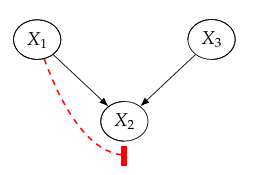
\includegraphics[width=\linewidth]{imgs/collider_nc.png} &
        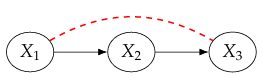
\includegraphics[width=\linewidth]{imgs/mediadora_nc.png} &
        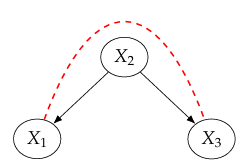
\includegraphics[width=\linewidth]{imgs/confusora_nc.png} \\
        
        \textbf{Condicionat} &
        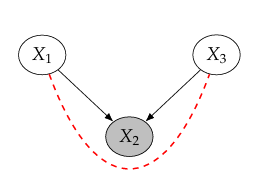
\includegraphics[width=\linewidth]{imgs/collider_c.png} &
        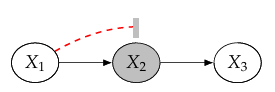
\includegraphics[width=\linewidth]{imgs/mediadora_c.png} &
        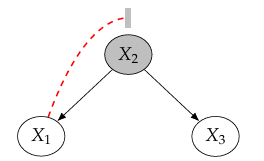
\includegraphics[width=\linewidth]{imgs/confusora_c.png} \\
        \bottomrule
        
        \end{tabular}
    \caption{Efectes del condicionament sobre diferents estructures causals. La línia roja discontinua representa el flux causal, les fletxes indiquen la direcció de la causalitat i els nodes grisos indiquen que s'ha condicionat la variable. De \cite{austin2011}}
    \label{taula:path}
    \end{table}

    Amb els tres casos que apareixen a la taula \ref{taula:path} podem entendre com flueix o s'interromp la dependència (i, potencialment, la causalitat) entre variables dins un DAG. Condicionar o no sobre determinades variables pot obrir o bloquejar camins causals, fet que té implicacions directes sobre la validesa de les nostres inferències.\par
    Ens interessarà mantenir oberts els camins que transmeten l'efecte causal real, com els que passen per variables mediadores, ja que connecten directament la intervenció amb l’outcome. En canvi, haurem de bloquejar els camins que introdueixen biaix, especialment aquells generats per variables confusores. També cal tenir molta cura amb els colliders, ja que condicionar sobre ells pot obrir camins espuris, fent que apareguin relacions que semblen causals però no ho són realment. Tot i això, en alguns contextos pot ser útil obrir aquests camins, ja que ens poden permetre explorar mecanismes ocults o efectes indirectes d’una variable sobre l’outcome.

    \subsection{Variables confusores}
    Els casos dels colliders i de les variables mediadores són especialment útils per entendre com podem bloquejar alguns camins causals o obrir-ne d’altres, segons les variables sobre les quals condicionem. No obstant això, el cas més preocupant en inferència causal és la presència de variables confusores no mesurades o no condicionades, ja que poden introduir biaixos greus en les estimacions. Aquest problema es pot il·lustrar fàcilment amb un diagrama com el següent:
    \begin{figure}[h]
        \centering        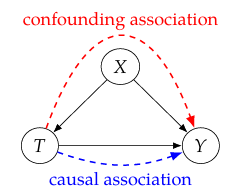
\includegraphics[width=0.3\linewidth]{imgs/confusora.png}
        \caption{DAG de tres variables amb X com variable confusora. De \cite{austin2011}}
        \label{fig:confusora}
    \end{figure}
    Ens situem en el cas en què tenim una variable de tractament T i volem estimar el seu efecte sobre una variable de resultat Y. Tanmateix, apareix una tercera variable X que actua com a confusora, ja que està relacionada tant amb T com amb Y. Aquesta relació pot introduir un biaix en l’estimació de l’efecte causal. Per tal de bloquejar aquest flux d’associació espúria i aïllar l’efecte causal de T sobre Y, cal condicionar sobre X, és a dir, controlar-la estadísticament.
    
\end{document}